\chapter{Diagrama de Casos de Uso}

\paragraph{}

Como é visivel na \prettyref{fig:casos_de_uso}, para este trabalho, foram definidos 5 casos de uso, sendo um para cada tipo de actores e dois que, apesar de terem características específicas para cada tipo de actor são comuns aos três.\\
Todos os tipos de utilizador podem efectuar login/logout, bem como listar as suas avaliações por datas e visualizar os detalhes das mesmas num dia escolhido.\\
O docente pode também marcar ou cancelar uma avaliação de uma disciplina por ele leccionada, enquanto que o aluno pode inscrever-se ou cancelar a inscrição numa avaliação de uma disciplina em que esteja matriculado. Por fim o coordenador pode validar ou cancelar a validação de uma avaliação de um curso que coordene.

\begin{figure}[!htbp]
\centering
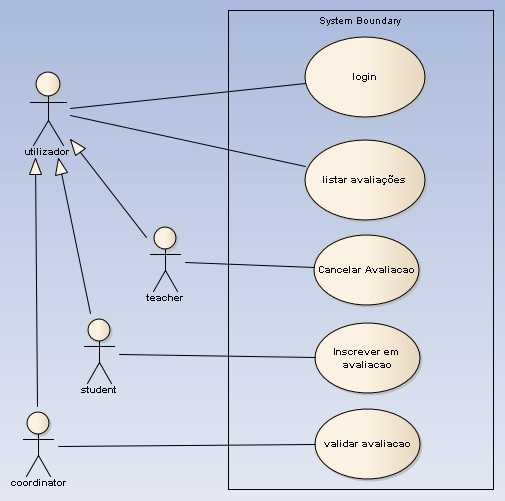
\includegraphics{imagens/casos_de_uso.jpg}
\caption{Diagrama: Casos de Uso}
\label{fig:casos_de_uso}
\end{figure}